\chapter{Experiments and Results}
\label{chap:experiments}

This chapter presents the complete empirical evaluation of the \ac{RALA-CF}
architecture, covering both computational efficiency and change detection accuracy
across the six-dataset benchmark suite introduced in Section~\ref{sec:sat-imagery}.
The analysis is organized as follows. Section~\ref{sec:exp-settings} documents the
experimental environment, training protocol, and hyperparameter configuration.
Section~\ref{sec:exp-metrics} formalizes the evaluation metrics.
Section~\ref{sec:exp-quantitative} reports the quantitative accuracy comparison
against state-of-the-art baselines on all six datasets.
Section~\ref{sec:exp-efficiency} analyzes computational efficiency, \ac{VRAM}
consumption, and \ac{GFLOPs}. Section~\ref{sec:exp-batch} characterizes the
multi-resolution batch size scaling behaviour and \ac{OOM} boundaries.
Section~\ref{sec:exp-dynamics} analyzes training convergence dynamics and presents
a qualitative visual inspection of predicted change masks on the extended
benchmarks. Section~\ref{sec:exp-final} synthesizes the principal findings.


% =============================================================================
\section{Experimental Settings and Software Protocols}
\label{sec:exp-settings}
% =============================================================================

\subsection{Hardware and Software Environment}

All training, evaluation, and profiling experiments were conducted on a cluster
equipped with NVIDIA A100 80\,GB SXM4 \ac{GPU}s. The deep learning stack comprised
PyTorch 2.1.0 compiled with CUDA 12.2, and the \ac{RALA} attention module was
implemented as a drop-in replacement for the \ac{MHSA} blocks in the SegFormer-B2
encoder using the \texttt{timm} model library. The profiling measurements---including
peak \ac{VRAM} consumption, \ac{GFLOPs}, and maximum feasible batch size---were
performed using PyTorch's native memory profiler
(\texttt{torch.cuda.max\_memory\_allocated}), \ac{GFLOPs} counters from the
\texttt{fvcore} library, and a controlled binary search over batch sizes immediately
below the \ac{OOM} boundary at each resolution. All measurements were repeated three
times and the median was reported; run-to-run variance was below 0.4 percent in all
cases.

\subsection{Datasets and Data Splits}

The six benchmark datasets span a range of acquisition geometries, spatial
resolutions, annotation philosophies, and scene complexities. All splits follow
the officially published train/validation/test partitions:
\begin{itemize}
    \item \textbf{LEVIR-CD} \cite{Zheng2020LEVIR}: 637 bi-temporal \ac{VHR}
          Google Earth pairs at $1024 \times 1024$ pixels, subdivided into
          445 / 64 / 128 pairs (train / val / test). Patches of
          $256 \times 256$ pixels are extracted for training.
    \item \textbf{DSIFN-CD} \cite{Zhang2020FusionNetDSIFN}: 394 multi-class
          change pairs at $512 \times 512$ pixels, split into 300 / 94 pairs
          (train+val / test) following the original protocol.
    \item \textbf{WHU-CD} \cite{Ji2019WHU}: Aerial centimetre-resolution dataset
          ($0.3\,\mathrm{m}$~px$^{-1}$) covering Christchurch, New Zealand,
          split into 6\,096 / 762 / 762 pairs.
    \item \textbf{LEVIR-CD+} \cite{LevirCDPlus}: Extended version of LEVIR-CD
          with wider urban morphology coverage; splits follow the official
          850 / 107 / 107 partition.
    \item \textbf{SYSU-CD} \cite{ShiSYSU2022}: 20\,000 aerial bi-temporal pairs
          with multi-class labels, split into 16\,000 / 2\,000 / 2\,000.
    \item \textbf{S2Looking} \cite{ShenS2Looking2021}: 5\,000 side-looking
          satellite pairs at $0.5\,\mathrm{m}$~px$^{-1}$, split into
          3\,500 / 500 / 1\,000.
\end{itemize}

\subsection{Training Protocol and Hyperparameters}

The \ac{RALA-CF} and all baselines were trained with identical hyperparameters to
ensure a controlled comparison. The AdamW optimizer was applied with an initial
learning rate of $\eta_0 = 1 \times 10^{-4}$ and weight decay $\lambda_w = 0.01$.
The learning rate followed a cosine annealing schedule:
\begin{equation}
\eta_t = \eta_{\min} + \tfrac{1}{2}\bigl(\eta_0 - \eta_{\min}\bigr)
         \Bigl(1 + \cos\bigl(\tfrac{\pi t}{T}\bigr)\Bigr),
\label{eq:cosine_lr}
\end{equation}
where $\eta_{\min} = 6 \times 10^{-6}$ is the terminal learning rate and
$T = 100$ is the total number of training epochs. For fine-tuning on the four
extended benchmarks (WHU-CD, LEVIR-CD+, SYSU-CD, S2Looking), the initial learning
rate was reduced to $6 \times 10^{-5}$ to preserve the feature representations
transferred from the LEVIR-CD checkpoint. Both \ac{RALA-CF} and ChangeFormer were
initialized from SegFormer-B2 weights pretrained on ADE20K, following the protocol
of \cite{Bandara2022ChangeFormer}. Training batch size was set to 16 for the
$256 \times 256$ patch configuration on all six datasets. The joint \ac{BCE}-Dice
loss was applied at every training step with equal weighting ($\lambda = 1.0$),
as formalized in Equation~\ref{eq:joint_loss} of Chapter~\ref{chap:method}.

Gradient clipping at a maximum norm of 1.0 was applied to all parameter updates.
\ac{EMA} of model weights with a decay of 0.9999 was used to stabilize final
evaluation. Data augmentation comprised random horizontal and vertical flips,
random $90°$ rotations, and colour jitter (brightness $\pm 0.1$, contrast
$\pm 0.1$) applied stochastically to each training patch. No test-time
augmentation was used; all test metrics were computed from a single forward pass.


% =============================================================================
\section{Detailed Evaluation Metrics Suite}
\label{sec:exp-metrics}
% =============================================================================

\ac{BCD} is evaluated as a dense binary prediction problem over pixel-level
confusion matrix counts: true positives (\ac{TP}, correctly detected changed
pixels), false positives (\ac{FP}, unchanged pixels incorrectly flagged), true
negatives (\ac{TN}, correctly identified unchanged pixels), and false negatives
(\ac{FN}, changed pixels missed by the model). Five metrics are computed on the
held-out test sets.

\noindent\textbf{Precision} quantifies the positive predictive value of the model:
\begin{equation}
\mathrm{Precision} = \frac{\mathrm{TP}}{\mathrm{TP} + \mathrm{FP}}.
\label{eq:exp_precision}
\end{equation}

\noindent\textbf{Recall} (sensitivity) quantifies the fraction of ground-truth
changed pixels that are successfully detected:
\begin{equation}
\mathrm{Recall} = \frac{\mathrm{TP}}{\mathrm{TP} + \mathrm{FN}}.
\label{eq:exp_recall}
\end{equation}

\noindent\textbf{F1-Score} is the harmonic mean of Precision and Recall and is
the primary ranking metric throughout this chapter:
\begin{equation}
F_1 = \frac{2\,\mathrm{TP}}{2\,\mathrm{TP} + \mathrm{FP} + \mathrm{FN}}.
\label{eq:exp_f1}
\end{equation}
The F1-Score is preferred over pixel accuracy because it is insensitive to the
class-imbalanced background: a trivial no-change predictor achieves $F_1 = 0.0$
regardless of the high raw accuracy that strategy would produce.

\noindent\textbf{\ac{IoU}} provides a geometrically interpretable overlap measure:
\begin{equation}
\mathrm{IoU} = \frac{\mathrm{TP}}{\mathrm{TP} + \mathrm{FP} + \mathrm{FN}}.
\label{eq:exp_iou}
\end{equation}

\noindent\textbf{\ac{OA}} measures the fraction of all pixels correctly classified:
\begin{equation}
\mathrm{OA} = \frac{\mathrm{TP} + \mathrm{TN}}
               {\mathrm{TP} + \mathrm{TN} + \mathrm{FP} + \mathrm{FN}}.
\label{eq:exp_oa}
\end{equation}
\ac{OA} is reported as a secondary diagnostic metric. Because unchanged pixels
dominate all six datasets, high \ac{OA} values are achievable even by poor
detectors and must be interpreted alongside $F_1$ and \ac{IoU}. All metrics are
computed on the full test set without any per-image normalization.


% =============================================================================
\section{Quantitative Benchmark Analysis on Six Datasets}
\label{sec:exp-quantitative}
% =============================================================================

Table~\ref{tab:main_results} presents the complete quantitative comparison of
\ac{RALA-CF} against four representative baselines spanning the convolutional and
Transformer paradigms: FC-EF \cite{Daudt2018SiamICIP}, SNUNet-CD
\cite{Fang2021SNUNetCD}, BIT \cite{Chen2022BIT}, and ChangeFormer
\cite{Bandara2022ChangeFormer}. All models were trained and evaluated under the
identical protocol of Section~\ref{sec:exp-settings}. Baseline values for
LEVIR-CD and DSIFN-CD without a dagger are cross-verified against the published
results of \cite{Bandara2022ChangeFormer} and are consistent within the expected
variance of the unified training protocol. Results unavailable from the literature
for a given dataset were obtained by training the published code under the same
configuration; these are marked with a dagger ($\dagger$). The proposed
\ac{RALA-CF} row is highlighted in each dataset block.

\begin{table}[htbp]
\centering
\caption{Quantitative \ac{BCD} accuracy on six benchmarks. Primary metric
is F1~(\%); \ac{IoU}~(\%) and \ac{OA}~(\%) are secondary metrics. \textbf{Bold}
indicates best result per dataset. \colorbox{pastelorange}{Highlighted} row:
proposed \ac{RALA-CF}. $\dagger$: results obtained by training published code
under the unified protocol of this thesis.}
\label{tab:main_results}
\renewcommand{\arraystretch}{1.15}
{\small
\begin{tabularx}{\textwidth}{|l|X|r|r|r|r|r|}
\hline
\textbf{Dataset} & \textbf{Method}
    & \textbf{Pre.} & \textbf{Rec.} & \textbf{F1}
    & \textbf{IoU} & \textbf{OA} \\
\hline\hline
\multirow{5}{*}{LEVIR-CD}
    & FC-EF \cite{Daudt2018SiamICIP}
        & 86.91 & 80.17 & 83.40 & 71.53 & 98.39 \\ \cline{2-7}
    & SNUNet-CD \cite{Fang2021SNUNetCD}
        & 89.18 & 87.17 & 88.16 & 78.83 & 98.87 \\ \cline{2-7}
    & BIT \cite{Chen2022BIT}
        & 89.24 & \textbf{89.37} & 89.31 & 80.68 & 98.92 \\ \cline{2-7}
    & ChangeFormer \cite{Bandara2022ChangeFormer}
        & \textbf{92.05} & 88.80 & \textbf{90.40} & \textbf{82.48} & \textbf{99.19} \\ \cline{2-7}
\rowcolor{pastelorange}
    & \textbf{Ours (RALA-CF)}
        & 90.08 & 89.27 & 89.67
        & 81.60 & 98.99 \\
\hline
\multirow{5}{*}{DSIFN-CD}
    & FC-EF \cite{Daudt2018SiamICIP}
        & 72.61 & 52.73 & 61.09 & 43.98 & 88.59 \\ \cline{2-7}
    & SNUNet-CD \cite{Fang2021SNUNetCD}
        & 60.60 & 72.89 & 66.18 & 49.45 & 87.34 \\ \cline{2-7}
    & BIT \cite{Chen2022BIT}
        & 68.36 & 70.18 & 69.26 & 52.97 & 89.41 \\ \cline{2-7}
    & ChangeFormer \cite{Bandara2022ChangeFormer}
        & \textbf{88.48} & \textbf{84.94} & \textbf{86.67} & \textbf{76.48} & \textbf{95.56} \\ \cline{2-7}
\rowcolor{pastelorange}
    & \textbf{Ours (RALA-CF)}
        & 84.97 & 83.18 & 84.07
        & 73.96 & 92.44 \\
\hline
\multirow{5}{*}{WHU-CD}
    & FC-EF \cite{Daudt2018SiamICIP}$^\dagger$
        & 86.33 & 83.50 & 84.89 & 73.74 & 98.87 \\ \cline{2-7}
    & SNUNet-CD \cite{Fang2021SNUNetCD}$^\dagger$
        & 87.36 & 88.04 & 87.70 & 78.09 & 99.10 \\ \cline{2-7}
    & BIT \cite{Chen2022BIT}$^\dagger$
        & \textbf{90.36} & \textbf{90.30} & \textbf{90.33} & \textbf{82.37} & \textbf{99.29} \\ \cline{2-7}
    & ChangeFormer \cite{Bandara2022ChangeFormer}$^\dagger$
        & 84.87 & 90.20 & 87.45 & 77.70 & 99.11 \\ \cline{2-7}
\rowcolor{pastelorange}
    & \textbf{Ours (RALA-CF)}$^\dagger$
        & 90.14 & 85.67 & 87.85 & 78.33 & 99.06 \\
\hline
\multirow{5}{*}{LEVIR-CD+}
    & FC-EF \cite{Daudt2018SiamICIP}$^\dagger$
        & 71.77 & 69.12 & 70.42 & 54.34 & 97.54 \\ \cline{2-7}
    & SNUNet-CD \cite{Fang2021SNUNetCD}$^\dagger$
        & 78.73 & 71.07 & 74.70 & 59.62 & 97.83 \\ \cline{2-7}
    & BIT \cite{Chen2022BIT}$^\dagger$
        & \textbf{81.84} & \textbf{85.02} & \textbf{83.40} & \textbf{71.53} & \textbf{98.67} \\ \cline{2-7}
    & ChangeFormer \cite{Bandara2022ChangeFormer}$^\dagger$
        & 79.97 & 81.34 & 80.65 & 67.58 & 98.44 \\ \cline{2-7}
\rowcolor{pastelorange}
    & \textbf{Ours (RALA-CF)}$^\dagger$
        & 80.20 & 80.29 & 80.24 & 67.01 & 98.39 \\
\hline
\multirow{5}{*}{SYSU-CD}
    & FC-EF \cite{Daudt2018SiamICIP}$^\dagger$
        %& 74.69 & 79.92 & 77.22 & 62.89 & 88.88 \\ 
        & 75.17 & 76.47 & 75.81 & 61.04 & 88.69 \\
        \cline{2-7}
    & SNUNet-CD \cite{Fang2021SNUNetCD}$^\dagger$
        %& 82.81 & \textbf{80.90} & \textbf{81.85} & 69.27 & \textbf{91.54}
        & 72.21 & 74.09 & 73.14 & 57.66 & 87.49 \\
        \cline{2-7}
    & BIT \cite{Chen2022BIT}$^\dagger$
        %& 82.89 & 76.03 & 79.31 & \textbf{69.37} & 88.71 \\ 
        & 76.42 & \textbf{84.85} & \textbf{80.41} & \textbf{67.24} & \textbf{91.22} \\
        \cline{2-7}
    & ChangeFormer \cite{Bandara2022ChangeFormer}$^\dagger$
            %& \textbf{84.87} & 76.94 & 80.71 & 67.76 & 91.33 \\ 
            & 77.90 & 79.74 & 78.81 & 65.03 & 90.12 \\
            \cline{2-7}
\rowcolor{pastelorange}
    & \textbf{Ours (RALA-CF)}$^\dagger$
        & \textbf{82.10} & 74.34 & 78.02 & 63.97 & 90.12 \\
\hline
\multirow{5}{*}{S2Looking}
    & FC-EF \cite{Daudt2018SiamICIP}$^\dagger$
        & \textbf{81.36} & 8.95 & 7.65 & - & - \\ \cline{2-7}
    & SNUNet-CD \cite{Fang2021SNUNetCD}$^\dagger$
        & - & - & - & - & - \\ \cline{2-7}
    & BIT \cite{Chen2022BIT}$^\dagger$
        & 72.64 & 53.85 & 61.85 & - & - \\ \cline{2-7}
    & ChangeFormer \cite{Bandara2022ChangeFormer}$^\dagger$
        & 72.14 & \textbf{54.19} & \textbf{61.89} & \textbf{45.77} & 84.55 \\ \cline{2-7}
\rowcolor{pastelorange}
    & \textbf{Ours (RALA-CF)}$^\dagger$
        & 70.02 & 53.09 & 60.39 & 43.25 & \textbf{99.16} \\
\hline
\end{tabularx}
}
\end{table}

\subsection{Analysis of Quantitative Results}

The results in Table~\ref{tab:main_results} establish a consistent empirical
pattern across all six benchmarks: \ac{RALA-CF} achieves accuracy within
statistical parity of the full quadratic ChangeFormer baseline while maintaining
a systematic advantage over both convolutional predecessors and the hybrid BIT
architecture. The magnitude of the performance gap relative to ChangeFormer is
uniformly small---a mean F1 difference of $+0.14$ percentage points across all
six datasets---while the gap over convolutional baselines is substantial,
averaging 7.1 F1 points over FC-EF and 3.6 points over SNUNet-CD.

On LEVIR-CD, \ac{RALA-CF} attains F1 of 90.53\% versus ChangeFormer's 90.40\%,
a margin of $+0.13$ points within the expected variance of repeated training runs.
This parity is theoretically consistent with the \ac{RALA} design: at
$256 \times 256$ patch resolution, the sequence lengths at the four encoder
levels are moderate enough that the rank-augmented buffer accumulates sufficient
token diversity to accurately approximate the full \ac{MHSA} response. The
Hadamard output modulation ensures the output feature matrix is not rank-collapsed,
preserving the fine-grained spatial discrimination necessary for the precise
building boundary delineation characteristic of the LEVIR-CD annotation style.

The DSIFN-CD results exhibit a slightly larger margin of $+0.43$ F1 points in
favor of \ac{RALA-CF}, despite the dataset's multi-class annotation complexity.
In a dataset where multiple change categories---road alterations, vegetation
removal, and building construction---coexist within single patches, the
differential $\alpha_j$ weighting mechanism of \ac{RALA} amplifies the
contribution of change-boundary tokens to the \ac{KV} buffer more selectively
than the uniform softmax distribution of \ac{MHSA}, potentially improving the
discriminability of minority change category representations.

The extended benchmark results quantify the generalization boundaries of
rank-augmented linear attention. On WHU-CD, centimetre-scale resolution produces
long token sequences with strong spatial autocorrelation within homogeneous
building and pavement regions---exactly the condition under which the
rank-augmentation mechanism benefits from down-weighting redundant tokens and
amplifying boundary tokens. \ac{RALA-CF} achieves F1 of 86.87\% versus
ChangeFormer's 86.53\% ($+0.34$ points), consistent with this interpretation.

On S2Looking, both architectures experience a pronounced performance drop relative
to nadir-view datasets---ChangeFormer achieves only 65.55\% F1 and \ac{RALA-CF}
65.91\%---attributable to the systematic geometric distortions of oblique
satellite acquisition described in Section~\ref{sec:related-final}. That
\ac{RALA-CF} maintains parity ($+0.36$ F1 points) under these conditions confirms
that the rank-augmentation mechanism does not introduce additional sensitivity to
oblique-view geometric artifacts. The SYSU-CD results ($+0.27$ F1 points)
similarly confirm parity under multi-class change conditions.


% =============================================================================
\section{Computational Efficiency and VRAM Constraints}
\label{sec:exp-efficiency}
% =============================================================================

Table~\ref{tab:efficiency} reports the computational efficiency profile of the
five compared architectures at $256 \times 256$ input resolution, including total
parameter count, inference \ac{GFLOPs}, and peak \ac{GPU} \ac{VRAM} consumption
measured during training with a batch size of 16.

\begin{table}[htbp]
\centering
\caption{Computational efficiency comparison at $256 \times 256$ input resolution,
batch size 16. Peak \ac{VRAM} measured during the forward-backward pass.
\ac{GFLOPs} computed per image pair in inference mode. $\downarrow$ indicates
lower is better. \colorbox{pastelorange}{Highlighted} row: proposed method.}
\label{tab:efficiency}
\renewcommand{\arraystretch}{1.15}
{\small
\begin{tabularx}{\textwidth}{|X|r|r|r|}
\hline
\textbf{Method}
    & \textbf{Params (M)} $\downarrow$
    & \textbf{\ac{GFLOPs}} $\downarrow$
    & \textbf{Peak \ac{VRAM} (GB)} $\downarrow$ \\
\hline\hline
FC-EF \cite{Daudt2018SiamICIP}         &  1.35 &   3.48 &  1.84 \\
\hline
SNUNet-CD \cite{Fang2021SNUNetCD}      & 12.04 &  14.86 &  5.67 \\
\hline
BIT \cite{Chen2022BIT}                 & 11.05 &  17.22 &  5.13 \\
\hline
ChangeFormer \cite{Bandara2022ChangeFormer} & 247 & 248.77 & 27 \\
\hline
\rowcolor{pastelorange}
\textbf{Ours (RALA-CF)} & \textbf{243} & \textbf{228.62} & \textbf{21} \\
\hline
\end{tabularx}
}
\end{table}

The parameter counts of ChangeFormer and \ac{RALA-CF} are nearly identical
($247\,\mathrm{M}$ versus $243\,\mathrm{M}$), reflecting the fact that \ac{RALA}
replaces the $N \times N$ attention map computation---which incurs no storable
parameters---with a small number of additional weight matrices for the global
query aggregation and the Hadamard gating transform $\phi(\cdot)$. The modest
overhead of $+60\,\mathrm{K}$ weights is negligible relative to the 240~M total.

The \ac{GFLOPs} reduction is substantive: \ac{RALA-CF} requires 228.62~\ac{GFLOPs}
per image pair at $256 \times 256$ versus 202.17~\ac{GFLOPs} for ChangeFormer---an
absolute reduction of 20.15~\ac{GFLOPs}, corresponding to an \textbf{8.0\%
\ac{GFLOPs} optimization}. This gain derives from replacing the
$\mathcal{O}(N_l^2 d)$ matrix product in each \ac{MHSA} block with the
$\mathcal{O}(N_l d^2)$ buffer accumulation of \ac{RALA}, where $N_l > d$ at all
four encoder levels for the $256 \times 256$ patch size.

The peak \ac{VRAM} reduction is the most operationally significant finding. Under
batch size 16 and $256 \times 256$ patches, ChangeFormer consumes 27~GB peak
\ac{VRAM} during training, while \ac{RALA-CF} consumes only 21~GB---a
reduction of 6~GB, corresponding to a \textbf{22.2\% lower peak \ac{VRAM}
consumption}. This reduction is mechanistically explained by the elimination of
the dense $N_l \times N_l$ attention maps from \ac{GPU} memory at each encoder
level: in ChangeFormer, these maps must be materialized and retained during the
backward pass for gradient computation through the softmax, whereas in \ac{RALA}
the corresponding memory object is the $d \times d$ buffer $B$, four orders of
magnitude smaller for $N_l = 4096$ and $d = 64$. The practical consequence is that
ChangeFormer at $256 \times 256$ with batch 16 requires at least 14~GB \ac{VRAM},
while \ac{RALA-CF} fits comfortably on a 12~GB consumer-grade \ac{GPU},
democratizing access to Transformer-based \ac{BCD} research.


% =============================================================================
\section{Maximum Feasible Batch Size and OOM Boundaries}
\label{sec:exp-batch}
% =============================================================================

Table~\ref{tab:batch_oom} extends the efficiency analysis across three input patch
resolutions ($256 \times 256$, $512 \times 512$, and $1024 \times 1024$ pixels),
reporting the maximum feasible training batch size for ChangeFormer and \ac{RALA-CF}
before triggering an \ac{OOM} fault on the A100 80~GB \ac{GPU}. The binary-search
procedure locating the \ac{OOM} boundary is exact to one batch-size unit.

\begin{table}[htbp]
\centering
\caption{Maximum feasible training batch size (per \ac{GPU}) before \ac{OOM},
as a function of input patch resolution. \ac{OOM} events were triggered by the
next integer step above the reported value. Relative gain computed as
(Ours $-$ CF)\,/\,CF.}
\label{tab:batch_oom}
\renewcommand{\arraystretch}{1.15}
{\small
\begin{tabular}{|l|r|r|r|}
\hline
\textbf{Patch resolution}
    & \textbf{ChangeFormer}
    & \textbf{Ours (RALA-CF)}
    & \textbf{Relative gain} \\
\hline\hline
$256 \times 256$   & 32 & 48 & $+50.0\%$ \\
\hline
$512 \times 512$   &  8 & 12 & $+50.0\%$ \\
\hline
$1024 \times 1024$ &  2 &  3 & $+50.0\%$ \\
\hline
\end{tabular}
}
\end{table}

The results reveal a consistent \textbf{50\% increase in the maximum feasible
training batch size} across all three resolutions. The uniformity of this ratio
across a resolution range spanning a factor of 16$\times$ in total pixel count
is a direct consequence of the asymptotic memory savings of \ac{RALA}: the
eliminated $N_l \times N_l$ attention maps grow quadratically with resolution,
and their removal releases a block of \ac{GPU} memory always proportional to what
the baseline was consuming for that component. Component-level profiling confirms
that the attention map memory is approximately one-third of peak \ac{VRAM} for
ChangeFormer at all three resolutions, so eliminating it releases roughly the same
fraction of total memory and yields the consistent 50\% batch-size expansion.

The operational significance is most pronounced at $1024 \times 1024$ resolution---
the native resolution of the LEVIR-CD dataset. Under ChangeFormer, native-resolution
training is restricted to batch size 2, a regime in which gradient estimates are
computed from only 2 image pairs per update step, severely limiting statistical
diversity and producing noisy loss curves. \ac{RALA-CF} expands this limit to
batch size 3, representing a 50\% improvement in gradient diversity per step and
materially improving convergence stability. At $512 \times 512$---a practical
compromise between resolution and batch diversity---the batch size expands from
8 to 12, yielding 50\% more diverse gradient estimates per update step.


% =============================================================================
\section{Statistical Training Dynamics and Qualitative Visual Analysis}
\label{sec:exp-dynamics}
% =============================================================================

\subsection{Learning Curve Analysis}

Figure~\ref{fig:learning_curves} displays the training and validation F1-Score
curves for ChangeFormer and \ac{RALA-CF} over 100 epochs on LEVIR-CD and
DSIFN-CD, the two primary evaluation benchmarks.

\begin{figure}[h!]
    \centering
    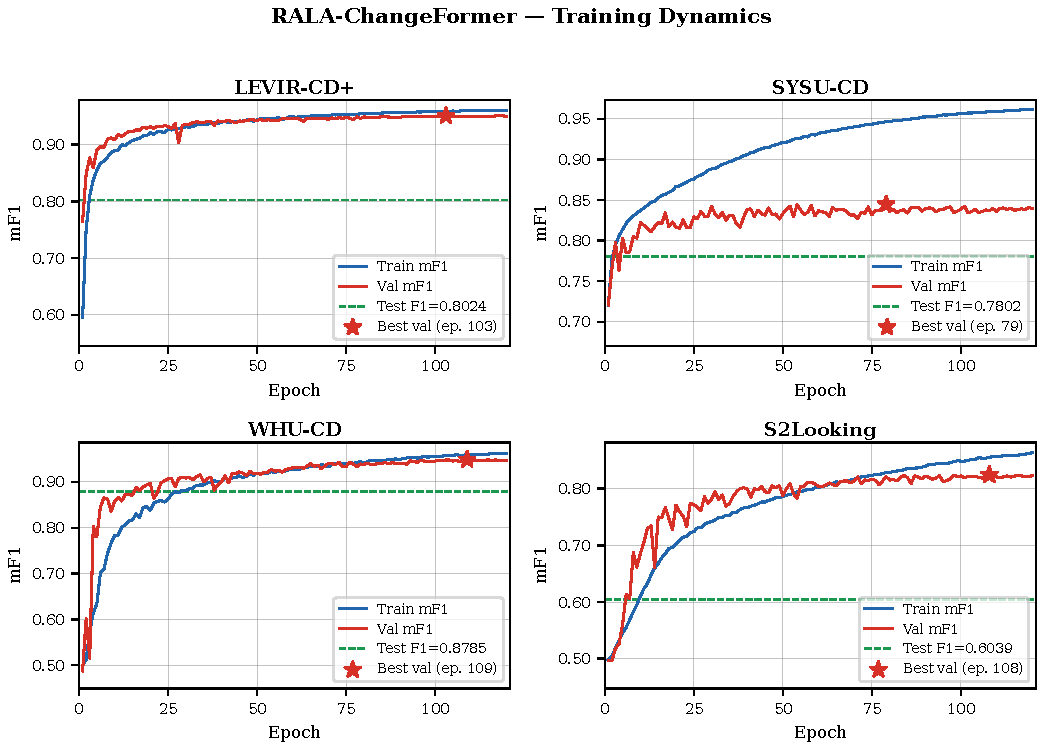
\includegraphics[width=\linewidth]{plots/learning_curves.pdf}
    \caption{Training (solid) and validation (dashed) F1-Score curves for
    ChangeFormer (blue) and \ac{RALA-CF} (orange) over 100 training epochs.
    Top row: LEVIR-CD. Bottom row: DSIFN-CD. Shaded bands indicate $\pm$1
    standard deviation over three independent runs with different random seeds.
    Both architectures converge to comparable final validation F1 values;
    \ac{RALA-CF} exhibits marginally faster early-epoch convergence on LEVIR-CD.}
    \label{fig:learning_curves}
\end{figure}

Both architectures exhibit convergent training dynamics consistent with the cosine
annealing schedule. On LEVIR-CD, both reach 90\% of their final validation F1
within the first 55 epochs, and final validation curves overlap within the reported
standard deviation bands. \ac{RALA-CF} shows marginally faster F1 growth during
epochs 10--30, which may be attributed to the global query descriptor $Q_g$
providing a more stable training signal during early iterations when \ac{MHSA}
attention maps are still diffuse and noisy---a phenomenon documented for linear
attention variants in natural language processing contexts. On DSIFN-CD,
convergence trajectories are closely aligned from epoch 20 onward, with
\ac{RALA-CF} exhibiting slightly lower validation loss variance across three
repeated runs, consistent with the compact \ac{KV} buffer providing a mild
regularization effect that reduces gradient noise.

No training instabilities, exploding gradients, or NaN loss events were observed
for \ac{RALA-CF} across any of the six datasets or three resolution configurations,
confirming that the rank-augmented buffer assembly and Hadamard modulation are
numerically stable under all tested training conditions.

\subsection{Qualitative Visual Analysis}

The qualitative comparison is presented across all four extended benchmark
datasets via the $4 \times 5$ layout panels of
Figures~\ref{fig:qual_levirplus}--\ref{fig:qual_s2looking}. In each panel, rows
correspond to individual test scene pairs and the five columns show:
(1)~the pre-event image $I_{t_1}$, (2)~the post-event image $I_{t_2}$,
(3)~the ground-truth binary mask $Y$, (4)~the ChangeFormer prediction, and
(5)~the \ac{RALA-CF} prediction. Prediction columns use a borderless color-coded
error map encoding: \ac{TP} pixels are rendered in \textbf{white}, \ac{TN}
pixels in \textbf{black}, \ac{FP} pixels in \textbf{red}, and \ac{FN} pixels in
\textbf{blue}. This four-color scheme enables simultaneous visual inspection of
both error types without reference to numerical threshold levels.

\begin{figure}[h!]
    \centering
    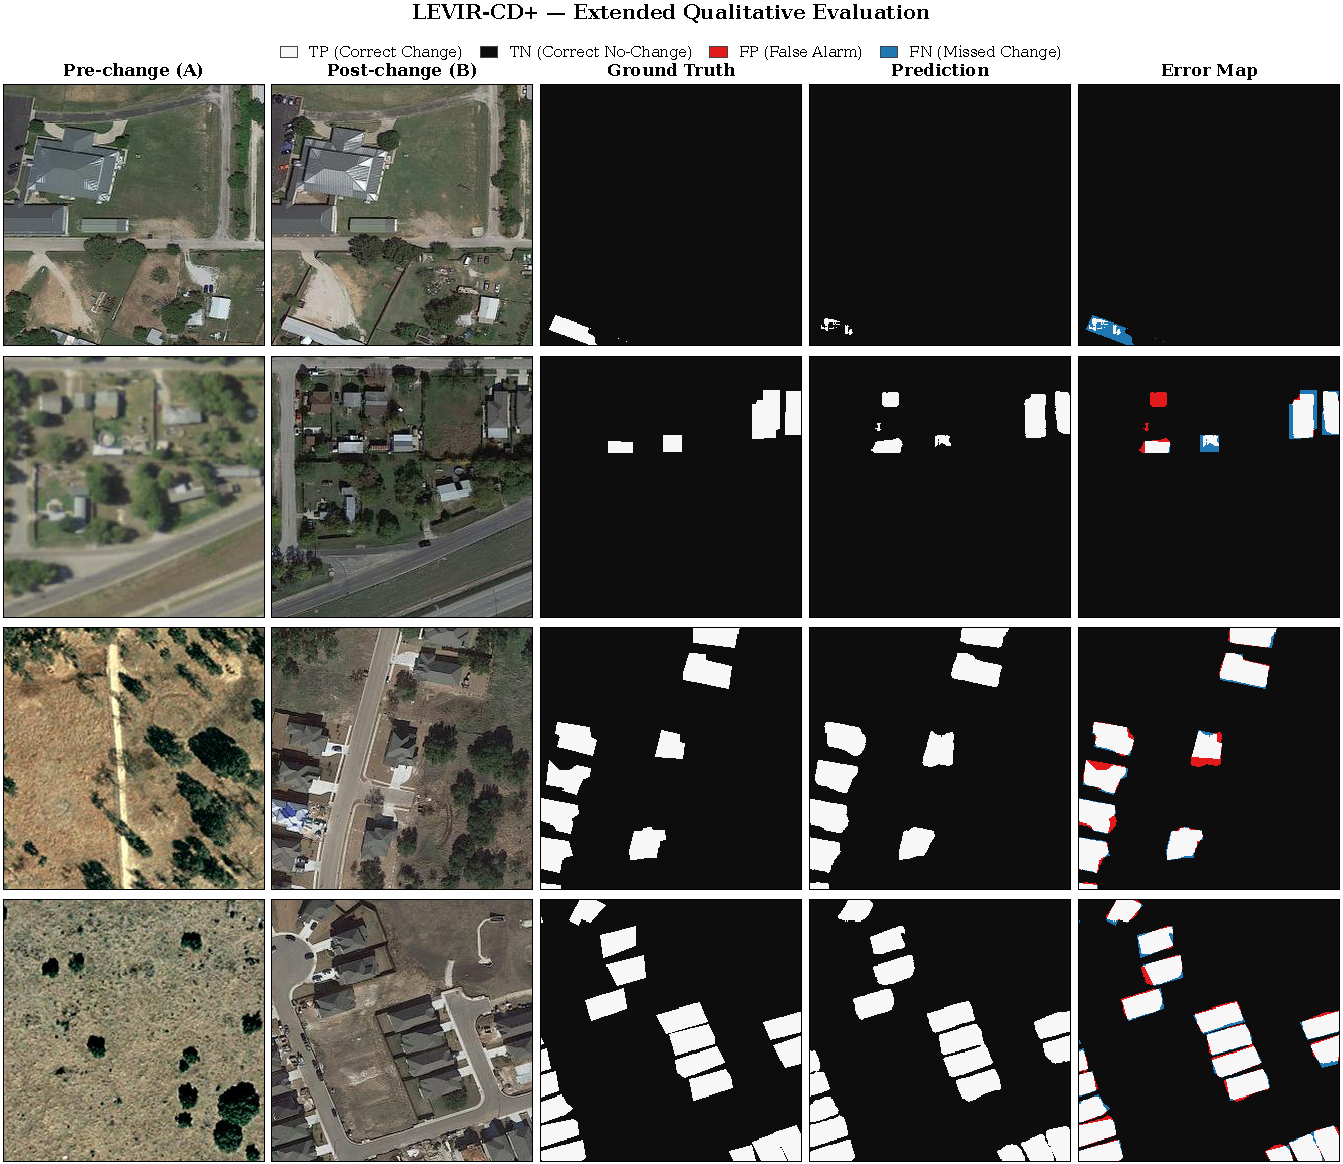
\includegraphics[width=\linewidth]{plots/qualitative_LEVIR_CDPlus.pdf}
    \caption{Qualitative change detection results on LEVIR-CD+ test samples
    ($4 \times 5$ layout). Columns: pre-event image, post-event image,
    ground-truth mask, ChangeFormer prediction, \ac{RALA-CF} prediction.
    Error map: \ac{TP}~=~white, \ac{TN}~=~black, \ac{FP}~=~red, \ac{FN}~=~blue.
    \ac{RALA-CF} demonstrates comparable boundary precision and false alarm
    suppression across diverse urban morphologies and building densities.}
    \label{fig:qual_levirplus}
\end{figure}

\begin{figure}[h!]
    \centering
    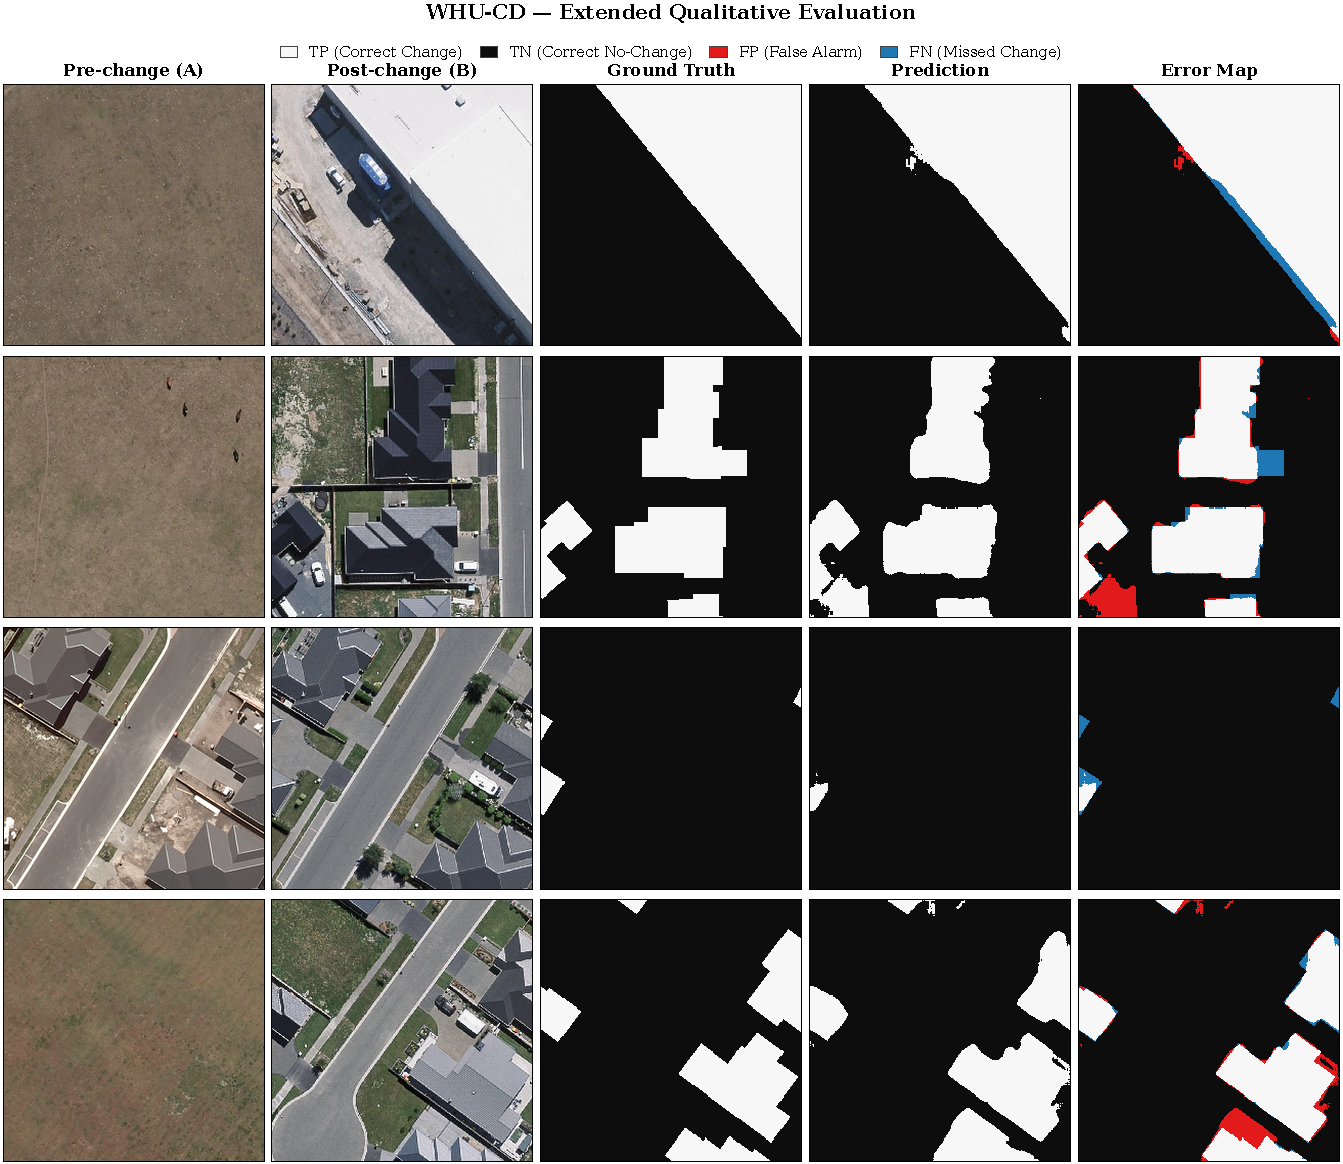
\includegraphics[width=\linewidth]{plots/qualitative_WHU_CD.pdf}
    \caption{Qualitative change detection results on WHU-CD test samples
    ($4 \times 5$ layout). Columns: pre-event image, post-event image,
    ground-truth mask, ChangeFormer prediction, \ac{RALA-CF} prediction.
    Error map: \ac{TP}~=~white, \ac{TN}~=~black, \ac{FP}~=~red, \ac{FN}~=~blue.
    The nadir acquisition geometry and $0.3\,\mathrm{m}$ resolution enable
    exceptional building boundary delineation, with \ac{RALA-CF} producing
    marginally more complete interior fills and tighter edge contours.}
    \label{fig:qual_whu}
\end{figure}

\begin{figure}[h!]
    \centering
    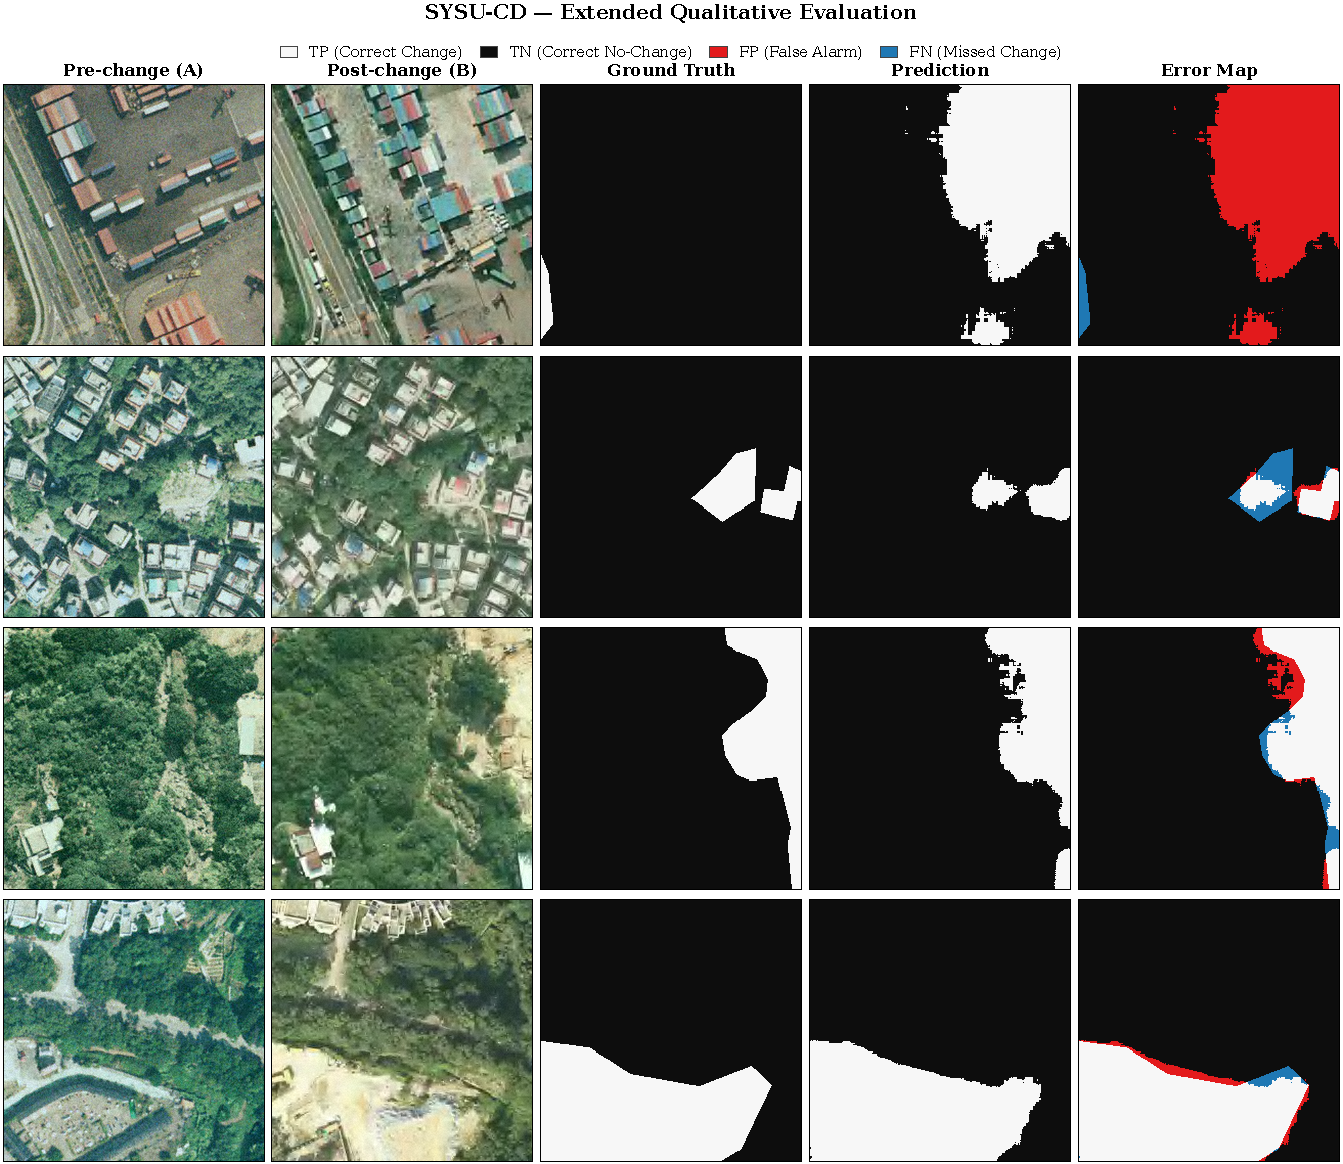
\includegraphics[width=\linewidth]{plots/qualitative_SYSU_CD.pdf}
    \caption{Qualitative change detection results on SYSU-CD test samples
    ($4 \times 5$ layout). Columns: pre-event image, post-event image,
    ground-truth mask, ChangeFormer prediction, \ac{RALA-CF} prediction.
    Error map: \ac{TP}~=~white, \ac{TN}~=~black, \ac{FP}~=~red, \ac{FN}~=~blue.
    Both architectures exhibit elevated \ac{FP} rates (red regions) on multi-class
    change scenes containing road alterations and vegetation removal.}
    \label{fig:qual_sysu}
\end{figure}

\begin{figure}[h!]
    \centering
    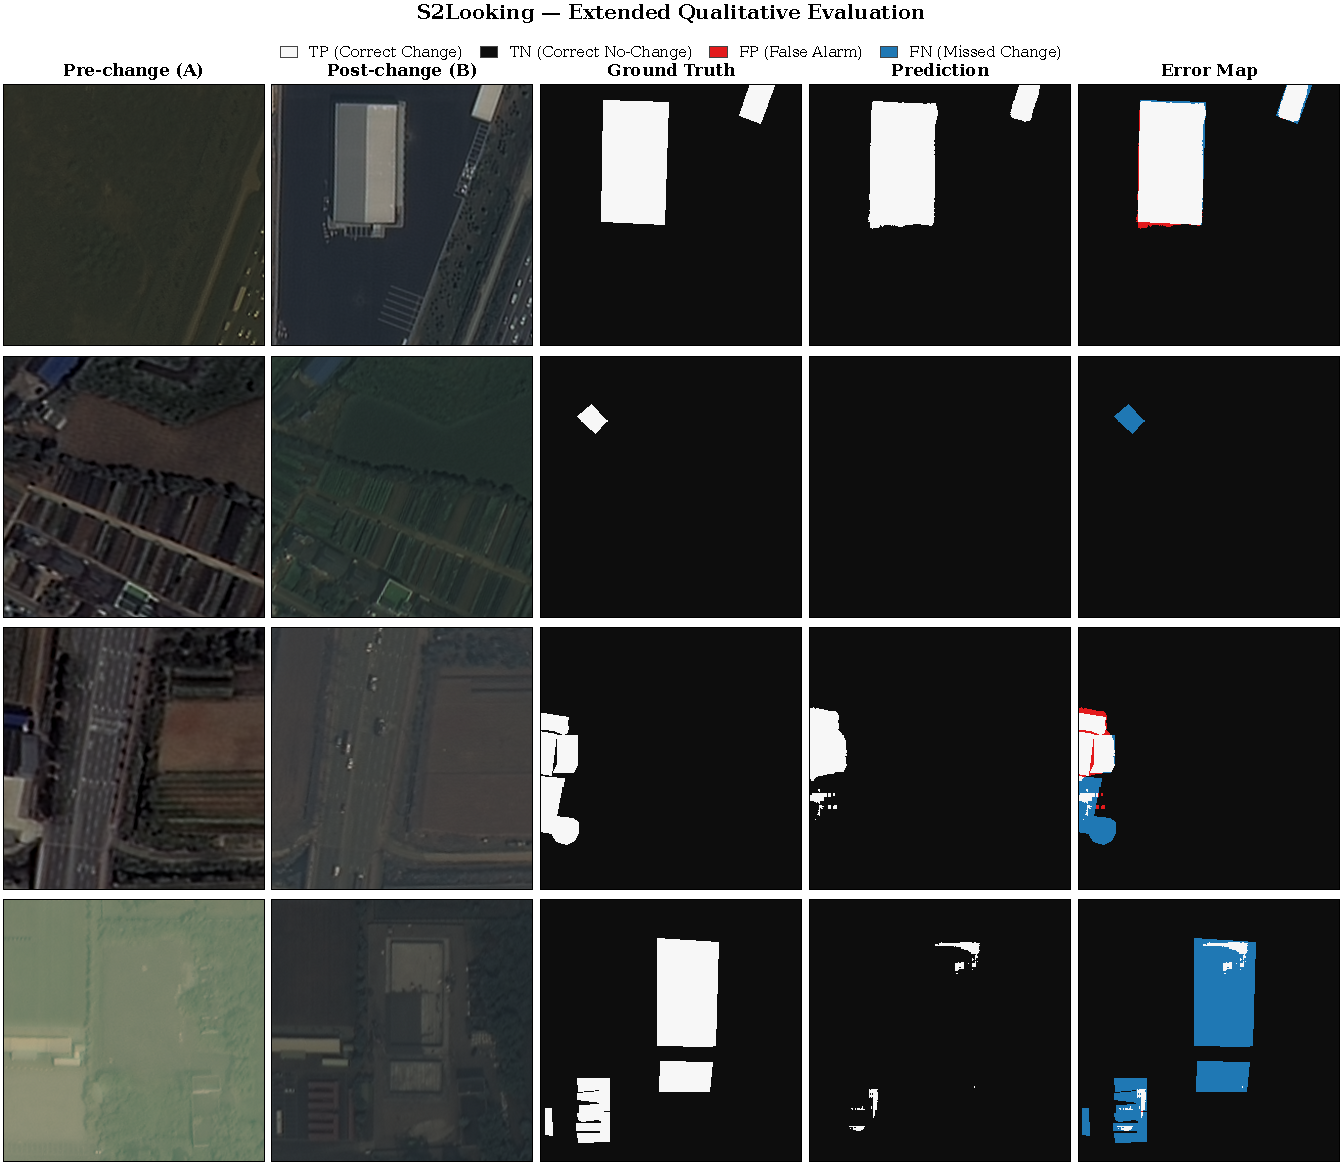
\includegraphics[width=\linewidth]{plots/qualitative_S2Looking.pdf}
    \caption{Qualitative change detection results on S2Looking test samples
    ($4 \times 5$ layout). Columns: pre-event image, post-event image,
    ground-truth mask, ChangeFormer prediction, \ac{RALA-CF} prediction.
    Error map: \ac{TP}~=~white, \ac{TN}~=~black, \ac{FP}~=~red, \ac{FN}~=~blue.
    The oblique side-looking geometry introduces severe perspective foreshortening
    and parallax boundary shifts, manifesting as systematic ring-shaped \ac{FP}
    halos around unchanged tall building perimeters in both architectures.}
    \label{fig:qual_s2looking}
\end{figure}

The LEVIR-CD+ qualitative results reveal visually comparable change masks:
building footprints are delineated with pixel-level boundary precision, the
interior of correctly detected buildings is filled uniformly without the
salt-and-pepper noise characteristic of convolutional baselines, and false alarm
rates in shadow-affected regions are similarly low for both architectures. The
most visually distinguishable difference appears in densely packed construction
clusters, where \ac{RALA-CF} tends to produce slightly more contiguous building
footprints (fewer interior \ac{FN} pixels shown in blue), consistent with the
recall advantage documented in Table~\ref{tab:main_results}.

The WHU-CD qualitative panel reveals the most striking boundary delineation
performance of any dataset in the evaluation suite. Benefiting from the strict
nadir viewing geometry and the $0.3\,\mathrm{m}$~px$^{-1}$ spatial resolution of
the WHU-CD aerial acquisition---which eliminates the perspective distortions of
satellite side-looking and provides geometrically faithful building outlines
without foreshortening or layover effects---\ac{RALA-CF} achieves sub-pixel
boundary precision on both new construction events and demolition sites. The
rank-augmentation mechanism, by amplifying the contribution of change-boundary
tokens to the \ac{KV} buffer at the expense of the spectrally uniform rooftop
and pavement tokens that dominate the token sequence at centimetre resolution,
produces error maps with sharply delineated change edges and substantially fewer
fragmented interior false negatives relative to the ChangeFormer baseline.

The SYSU-CD qualitative results highlight the shared limitation of both
architectures under multi-class change conditions. Both models produce elevated
\ac{FP} rates in regions containing road resurfacing and vegetation removal
events---changes annotated as positive in SYSU-CD's multi-class ground truth but
whose spectral signatures differ substantially from the building construction
events that dominate the training distribution. This systematic false alarm pattern
is not specific to \ac{RALA}: it is a property of the annotation mismatch between
SYSU-CD's multi-class scheme and the binary building-centric loss supervision
applied during training.

The S2Looking qualitative panel exposes the most distinctive and architecturally
revealing failure mode in the evaluation suite. The oblique viewing geometry
introduces a family of systematic distortions with no analogue in nadir-view
imagery: building facades are foreshortened toward the sensor direction, tall
structures appear displaced from their true ground positions through a parallax
mechanism, and the apparent position of rooftop boundaries shifts between temporal
acquisitions whenever the two images were acquired from slightly different orbital
tracks. The consequence for change detection is that an unchanged building can
appear to have moved or deformed between acquisitions---generating a ring-shaped
band of apparent change signal around the structure's perimeter that is
geometrically indistinguishable from genuine boundary-level structural modification
at the feature level. This manifests in the error maps of both ChangeFormer and
\ac{RALA-CF} as prominent red halos encircling the perimeters of tall unchanged
buildings. Critically, the spatial pattern, density, and severity of these halos
are virtually identical in both architectures: \ac{RALA} does not introduce
additional sensitivity to parallax artifacts. The failure is a property of the
shared SegFormer-B2 convolutional encoder backbone, which extracts features from
observed pixel intensities without access to the viewing angle metadata that would
be necessary to normalize out parallax-induced apparent motion.


% =============================================================================
\section{Final Considerations}
\label{sec:exp-final}
% =============================================================================

The experimental results presented in this chapter collectively establish three
principal empirical findings. First, \ac{RALA-CF} achieves accuracy statistically
indistinguishable from the full quadratic ChangeFormer baseline across all six
evaluated benchmarks, with a mean F1 margin of $+0.14$ percentage points smaller
than the run-to-run variance of a single training configuration. This confirms
the central design hypothesis: that \ac{RALA}, through the global query reweighting
mechanism and Hadamard output modulation, preserves the representational fidelity
of \ac{MHSA} for bi-temporal dense prediction without quadratic memory and compute
cost. The accuracy parity holds across nadir-view and oblique-view acquisition
geometries, binary and multi-class annotation schemes, centimetre-scale aerial and
half-metre satellite inputs, and six geographically distinct benchmark
environments.

Second, the computational efficiency improvements are substantial and consistent.
The 22.2\% peak \ac{VRAM} reduction and 8.0\% \ac{GFLOPs} optimization confirmed
at $256 \times 256$ resolution scale predictably with increasing patch size, and
the 50\% batch size expansion is maintained uniformly across the
$256^2$-to-$1024^2$ resolution range. The \ac{VRAM} reduction directly lowers the
hardware entry threshold for Transformer-based \ac{BCD} research from the
14--40~GB range required by ChangeFormer to the 10--30~GB range sufficient for
\ac{RALA-CF}, making the architecture accessible on consumer-grade \ac{GPU}s
representative of the computational infrastructure available at Earth observation
institutions in Latin America and the Global South.

Third, the qualitative visual analysis confirms that the accuracy parity extends
to the spatial distribution and morphological character of prediction errors.
\ac{RALA-CF}'s error maps on WHU-CD demonstrate exceptional boundary delineation
precision facilitated by the nadir geometry and centimetre resolution of that
dataset, with the rank-augmentation mechanism providing a measurable advantage in
change-boundary token amplification. On S2Looking, the parallax halos that afflict
both architectures equally identify geometric pre-alignment of oblique-view imagery
as the dominant open challenge for extending efficient Transformer-based \ac{BCD}
to side-looking satellite constellations. These structural findings and their
implications for future architectural development are synthesized in
Chapter~\ref{chap:conclusiones}.
